% Porting Wasm Semantics to ACL2 With Coding Agents
% ACL2 Workshop 2026 -- Ray Myers
% Reconstructed from the Canva deck; build with `make` (latexmk -pdf).

\documentclass[aspectratio=169,11pt]{beamer}

\usepackage[T1]{fontenc}
\usepackage[utf8]{inputenc}
\IfFileExists{FiraSans.sty}
  {\usepackage[scaled=.95]{FiraSans}\usepackage[scaled=.85]{FiraMono}}
  {\usepackage{tgheros}\usepackage{lmodern}\renewcommand{\sfdefault}{qhv}}
\renewcommand{\familydefault}{\sfdefault}
\usepackage{graphicx}
\usepackage{tikz}
\usetikzlibrary{positioning,arrows.meta,shapes.geometric,calc}
\usepackage{listings}
\usepackage{booktabs}
\usepackage{soul}
\usepackage{xcolor}

% ---------------------------------------------------------------- look
\definecolor{ink}{HTML}{1A1A1A}
\definecolor{muted}{HTML}{9A9A9A}
\definecolor{wasm}{HTML}{654FF0}   % WebAssembly purple
\definecolor{accent}{HTML}{1A0DAB} % link blue from the Canva deck
\definecolor{alert}{HTML}{E0393E}
\definecolor{codebg}{HTML}{F5F4F0}
\definecolor{boxbg}{HTML}{F4F3EF}
\definecolor{boxhl}{HTML}{E8F0FB}
\definecolor{boxhlb}{HTML}{4A86E8}
\definecolor{bar}{HTML}{2F6FD6}

\setbeamertemplate{navigation symbols}{}
\setbeamercolor{normal text}{fg=ink,bg=white}
\setbeamercolor{frametitle}{fg=ink}
\setbeamercolor{title}{fg=ink}
\setbeamercolor{structure}{fg=wasm}
\setbeamercolor{alerted text}{fg=alert}
\setbeamerfont{frametitle}{size=\LARGE,series=\mdseries}
\setbeamerfont{title}{size=\huge,series=\mdseries}
\setbeamertemplate{frametitle}{\vspace*{4mm}\centering\insertframetitle\par}
\setbeamertemplate{itemize item}{\color{wasm}\raisebox{.15ex}{\small$\bullet$}}
\setbeamertemplate{enumerate item}{\color{wasm}\insertenumlabel.}
\setbeamertemplate{footline}{%
  \hfill{\color{muted}\scriptsize\insertframenumber}\hspace*{4mm}\vspace*{3mm}}

% A slide that is just one or two centered statements.
\newcommand{\statement}[1]{%
  \vfill\begin{center}\LARGE #1\end{center}\vfill}
\newcommand{\muted}[1]{{\color{muted}#1}}
\newcommand{\link}[1]{{\color{accent}#1}}

% ---------------------------------------------------------------- code
\lstdefinestyle{acl2}{
  language=Lisp,
  basicstyle=\ttfamily\footnotesize,
  backgroundcolor=\color{codebg},
  frame=none, framesep=0pt, xleftmargin=4pt, xrightmargin=4pt,
  aboveskip=0pt, belowskip=0pt,
  keywordstyle=\color{ink},
  commentstyle=\color{muted},
  stringstyle=\color{alert!80!black},
  columns=fullflexible, keepspaces=true,
  escapeinside={(*@}{@*)},
  showstringspaces=false,
}
\lstdefinestyle{spectec}{
  style=acl2,
  basicstyle=\ttfamily\fontsize{6.6}{8}\selectfont,
  morekeywords={rule},
}
\newcommand{\hi}[1]{{\color{wasm}\bfseries #1}}

% ---------------------------------------------------------------- meta
\title{Porting Wasm Semantics to ACL2\\With Coding Agents}
\author{Ray Myers}
\institute{The Coding Agency}
\date{ACL2 Workshop 2026}

\begin{document}

% ================================================================ 1. Title
{\setbeamertemplate{footline}{}
\begin{frame}
  \vspace*{12mm}
  \begin{center}{\usebeamerfont{title}\inserttitle}\end{center}
  \vfill
  \begin{columns}[b]
    \column{.5\textwidth}
      {\Large Ray Myers}\\[1mm]
      \muted{The Coding Agency}
    \column{.4\textwidth}
      \raggedleft\large ACL2 Workshop 2026
  \end{columns}
  \vspace*{6mm}
\end{frame}}

% ================================================================ 2. Ported!
{\setbeamertemplate{footline}{}
\begin{frame}
  \vspace*{12mm}
  \begin{center}
    {\usebeamerfont{title}\color{muted}%
      \setstcolor{muted}\st{Porting} Wasm Semantics to ACL2\\With Coding Agents}
  \end{center}
  \vspace*{6mm}
  \begin{center}
    
\begin{tikzpicture}
      \node[rotate=8, text=accent, font=\Huge\bfseries\itshape] {Ported!};
    \end{tikzpicture}
  \end{center}
  \vfill
\end{frame}}

% ================================================================ 3. Why: proofs
\begin{frame}{Why?}
  \statement{Enable practical proofs of\\industrial software}
\end{frame}

% ================================================================ 4. Why: people/tools/agents
\begin{frame}{Why?}
  \begin{center}
  \begin{tikzpicture}[every node/.style={font=\LARGE}]
    \node (img) {
\includegraphics[height=3.6cm]{figs/handshake.png}};
    \node[left=1.2cm of img] {People};
    \node[right=1.2cm of img, align=center] {Coding\\Agents};
    \node[below=1mm of img] {Tools};
  \end{tikzpicture}
  \end{center}
\end{frame}

% ================================================================ 5. Question
\begin{frame}
  \statement{\huge Why bring Wasm semantics to ACL2\\using coding agents?}
\end{frame}

% ================================================================ 6. Wasm & ACL2
\begin{frame}
  \vfill
  \begin{minipage}{.8\textwidth}\LARGE
    \textbf{ACL2}\\
    Awesome industrial prover
    \\[6mm]
    \textbf{WebAssembly}\\
    Widely-deployed compilation target\\
    Official formal semantics
  \end{minipage}
  \vfill
\end{frame}

% ================================================================ 7. Coding Agent
\begin{frame}
  \vspace*{8mm}
  \begin{center}
    {\Huge Coding Agent}\\[1mm]
    \muted{\large (as currently conceived)}
  \end{center}
  \vspace*{6mm}
  \begin{center}\LARGE
    Language Model in a chat loop\\
    that calls tools for developing software
  \end{center}
  \vfill
\end{frame}

% ================================================================ 8. Toil
\begin{frame}
  \vspace*{14mm}
  \begin{center}\LARGE
    Semantics work is toilsome\\[6mm]
    Agents can help, \emph{given boundaries}
  \end{center}
  \begin{tikzpicture}[remember picture,overlay]
    \node[anchor=south east, inner sep=0] at (current page.south east)
      {
\includegraphics[height=3.4cm]{figs/sisyphus.png}};
  \end{tikzpicture}
\end{frame}

% ================================================================ 9-10. SpecTec
\begin{frame}
  \begin{center}
    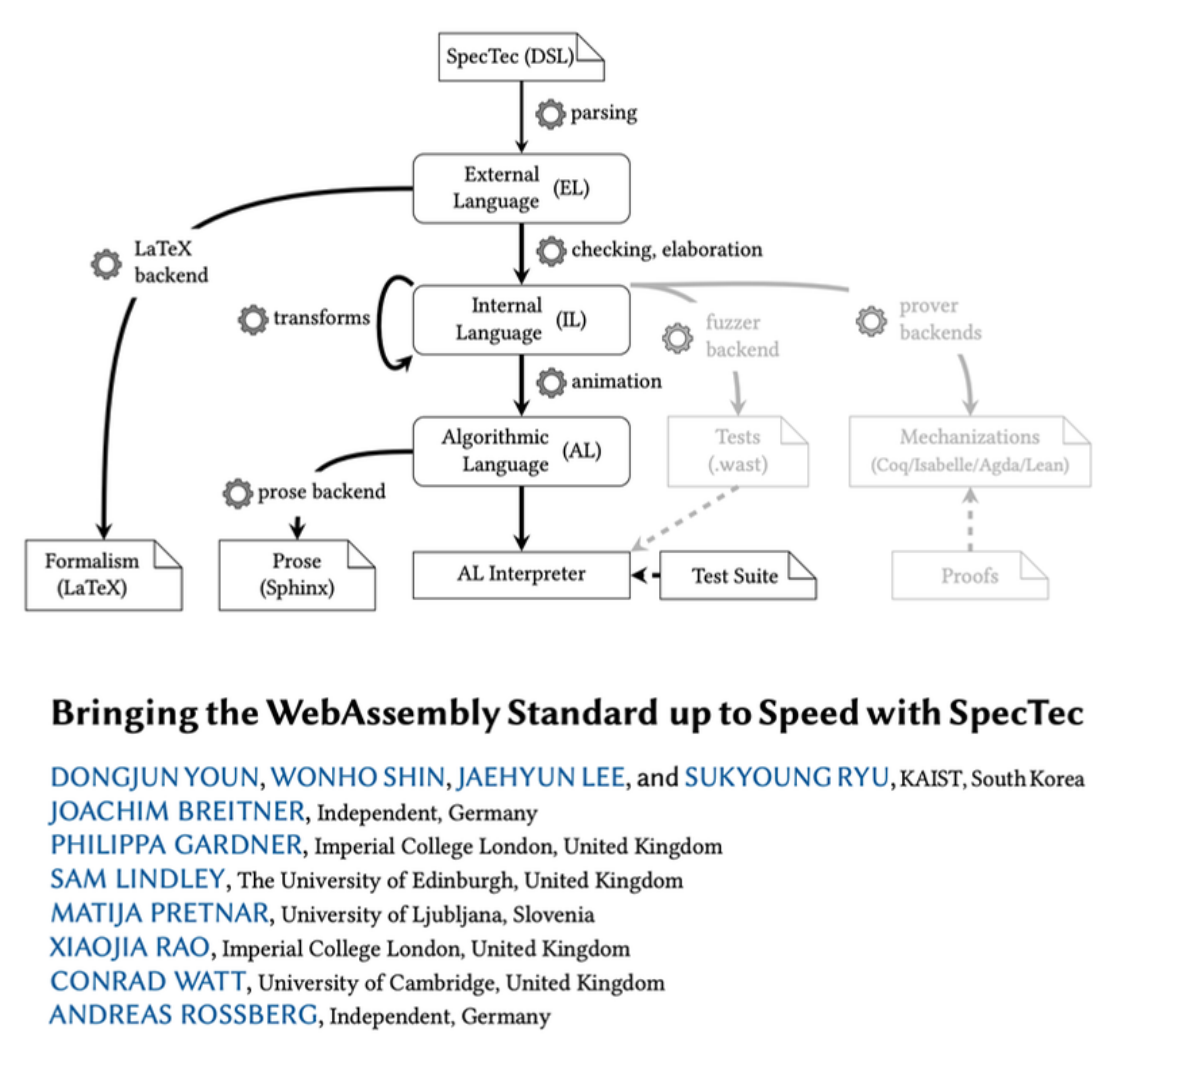
\includegraphics[height=.92\textheight]{figs/spectec-pipeline.png}
  \end{center}
\end{frame}

\begin{frame}
  \begin{center}
  \begin{tikzpicture}
    \node[inner sep=0, opacity=.55, anchor=south west] (img) at (0,0)
      {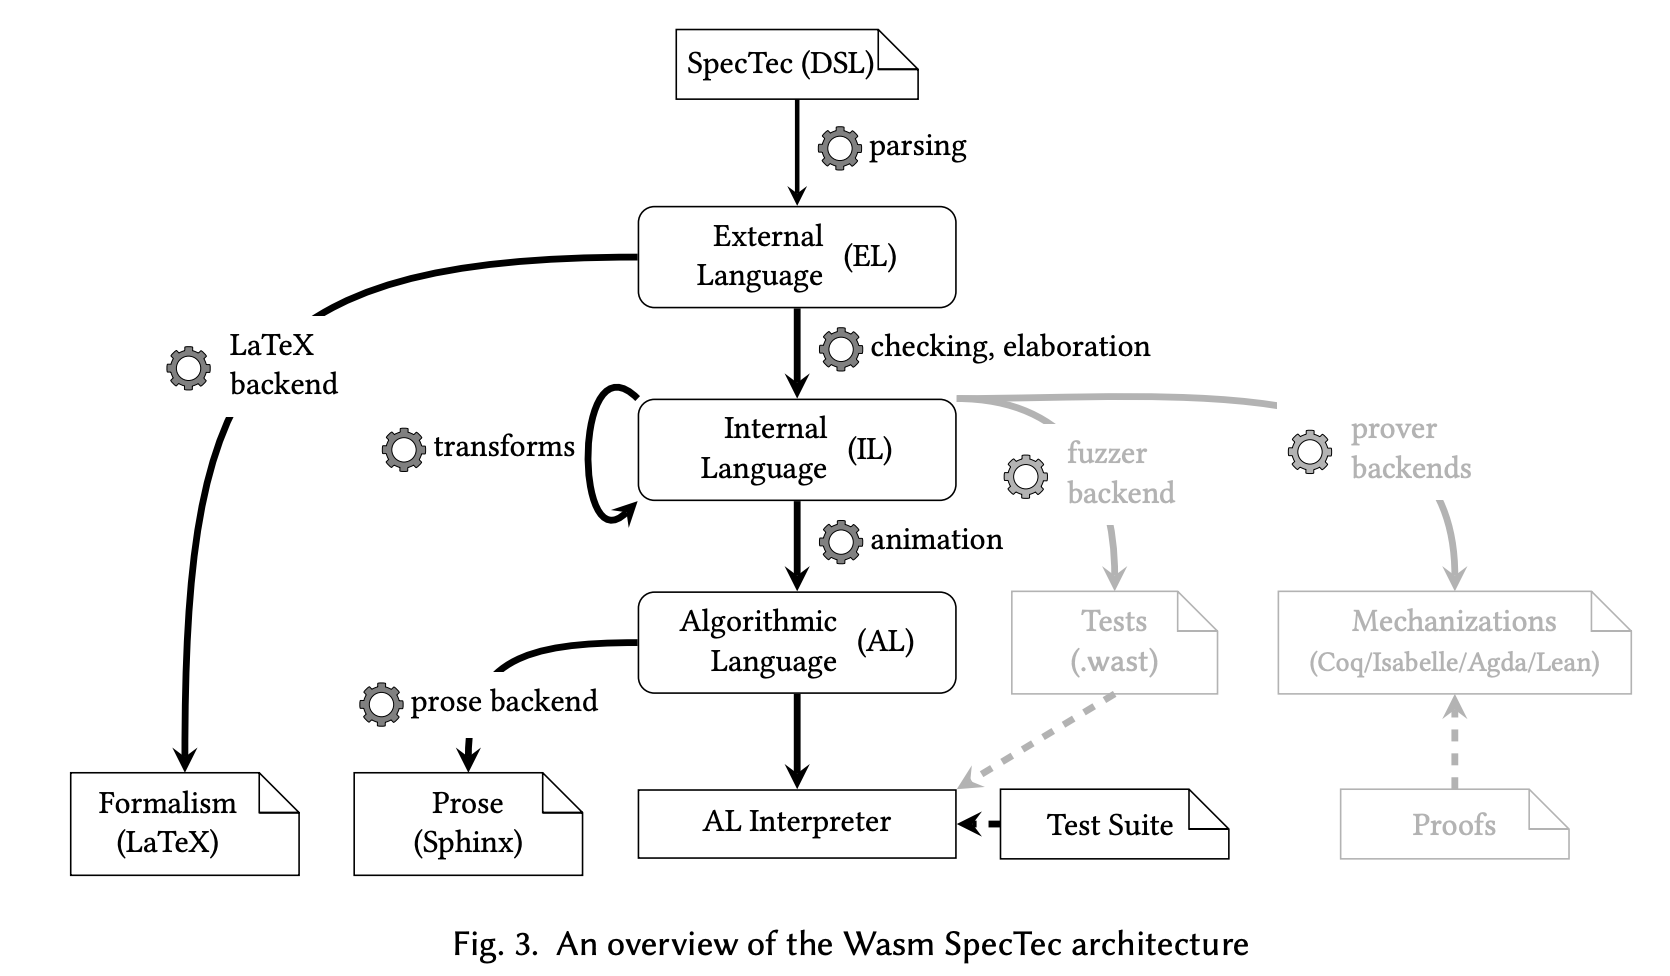
\includegraphics[width=.95\textwidth]{figs/spectec-diagram.png}};
    % coordinates as fractions of the image: (0,0) bottom left, (1,1) top right
    \begin{scope}[x={(img.south east)}, y={(img.north west)}]
      % circle the (greyed-out) "prover backends" box
      \draw[alert, line width=1.4pt] (.78,.50) ellipse [x radius=.085, y radius=.11];
      \node[alert, font=\bfseries, anchor=south] at (.78,.64) {ACL2 backend goes here};
    \end{scope}
  \end{tikzpicture}
  \end{center}
\end{frame}

% ================================================================ 11. Pipeline
\tikzset{
  stage/.style={draw=black!20, fill=boxbg, rounded corners=2pt,
                minimum width=2.4cm, minimum height=1.2cm,
                align=center, font=\scriptsize, inner sep=3pt},
  stagehl/.style={stage, draw=boxhlb, fill=boxhl, line width=.8pt},
  flow/.style={-{Stealth[length=2mm]}, black!60},
}
\newcommand{\pipeline}{%
  \node[stage] (spec) {\textbf{WebAssembly spec}\\[1pt]
    SpecTec source, 3.0\\25 files $\cdot$ 7,008 lines};
  \node[stage, right=11mm of spec] (il) {\textbf{SpecTec IL}\\[1pt]
    s-expressions\\pinned, checked in};
  \node[stagehl, right=6mm of il] (tr) {\textbf{il2acl2}\\[1pt]
    translator + runtime\\6,097 lines of ACL2};
  \node[stage, right=6mm of tr] (books) {\textbf{ACL2 books}\\[1pt]
    generated, certified\\218 / 218 reduction rules};
  \draw[flow] (spec) -- node[above=1pt, font=\tiny\ttfamily, black!60]{spectec} (il);
  \draw[flow] (il) -- (tr);
  \draw[flow] (tr) -- (books);
}

\begin{frame}{Pipeline}
  \begin{center}
  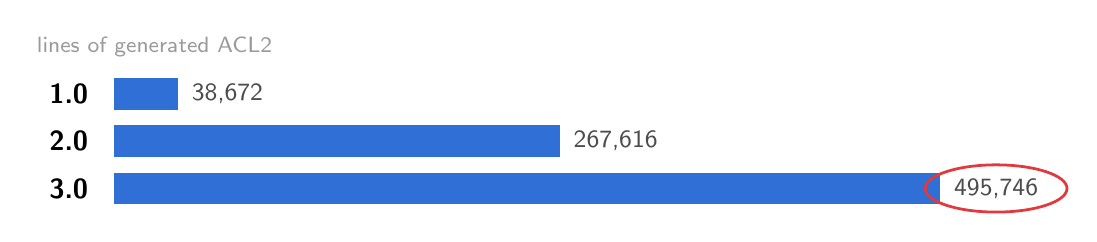
\begin{tikzpicture}
    \pipeline
    % lines of generated ACL2, by Wasm version
    \begin{scope}[yshift=-2.1cm, xshift=-1.2cm]
      \node[anchor=west, font=\footnotesize, muted] at (0,0) {lines of generated ACL2};
      \pgfmathsetmacro{\unit}{10.5/495.746}
      \foreach \v/\n/\lbl [count=\i] in
          {1.0/38.672/38{,}672, 2.0/267.616/267{,}616, 3.0/495.746/495{,}746} {
        \pgfmathsetmacro{\w}{\n*\unit}
        \node[anchor=east, font=\bfseries] at (.9,-.6*\i) {\v};
        \fill[bar] (1.1,-.6*\i-.2) rectangle ++(\w,.4);
        \node[anchor=west, font=\small, black!70] (lab\i) at (1.15+\w,-.6*\i) {\lbl};
      }
      \draw[alert, line width=1pt] (lab3) ellipse [x radius=.9cm, y radius=.3cm];
    \end{scope}
  \end{tikzpicture}
  \end{center}
\end{frame}

% ================================================================ 12. Trust base
\begin{frame}
  \vspace*{12mm}
  \begin{center}
  \begin{tikzpicture}
    \pipeline
    \draw[alert, line width=1.2pt] (tr) circle [radius=1.85cm];
  \end{tikzpicture}\\[10mm]
  {\LARGE Requires trusting $\approx$ 6K lines}
  \end{center}
  \vfill
\end{frame}

% ================================================================ 13. Rule: cleaned up
\begin{frame}[fragile]
  \vspace*{6mm}
  \begin{columns}[c]
    \column{.25\textwidth}
      \begin{center}\LARGE SpecTec rule\end{center}
    \column{.73\textwidth}
\begin{lstlisting}[style=spectec]
rule (*@\color{alert!80!black}Step\_pure/if-true@*):
  (CONST I32 c) ((*@\color{wasm}IF@*) bt instr_1* ELSE instr_2*)  ~>  (BLOCK bt instr_1*)
  -- if (*@\hi{c =/= 0}@*)
\end{lstlisting}
  \end{columns}
  \vspace*{5mm}
  \begin{columns}[c]
    \column{.25\textwidth}
      \begin{center}\LARGE ACL2 rule\\\muted{\large (cleaned up)}\end{center}
    \column{.73\textwidth}
\begin{lstlisting}[style=acl2]
(defun if-true (instrs)
  (case-match instrs
    (((:const (:i32) c) ((*@\hi{:ifelse}@*) bt then else))
     (and (true-listp then)
          (true-listp else)
          (*@\hi{(not (equal c 0))}@*)
          (list (list (list :block bt then)))))))
\end{lstlisting}
      \vspace*{2mm}
  \end{columns}
  \vfill
\end{frame}

% ================================================================ 14. Rule: as generated
\begin{frame}[fragile]
  \begin{columns}[c]
    \column{.25\textwidth}
      \begin{center}\LARGE SpecTec rule\\[22mm]
        Generated\\ACL2 rule\end{center}
    \column{.73\textwidth}
\begin{lstlisting}[style=spectec]
rule (*@\color{alert!80!black}Step\_pure/if-true@*):
  (CONST I32 c) ((*@\color{wasm}IF@*) bt instr_1* ELSE instr_2*)  ~>  (BLOCK bt instr_1*)
  -- if (*@\hi{c =/= 0}@*)
\end{lstlisting}
      \vspace*{2mm}
\begin{lstlisting}[style=acl2, basicstyle=\ttfamily\fontsize{4.6}{5.2}\selectfont]
(AND (TRUE-LISTP %A0)
     (EQUAL (ACL2::LEN %A0) 2)
     (LET* ((%T16 (CAR %A0)))
       (AND (CONSP %T16)
            (EQ (CAR %T16) :CONST)
            (TRUE-LISTP (CDR %T16))
            (EQUAL (ACL2::LEN (CDR %T16)) 2)
            (LET* ((%T17 (CAR (CDR %T16))))
              (AND (CONSP %T17)
                   (EQ (CAR %T17) :I32)
                   (TRUE-LISTP (CDR %T17))
                   (EQUAL (ACL2::LEN (CDR %T17)) 0)
                   (LET* ((C (CAR (CDR (CDR %T16))))
                          (%T18 (CAR (CDR %A0))))
                     (AND (CONSP %T18)
                          (EQ (CAR %T18) (*@\hi{:IFELSE}@*))
                          (TRUE-LISTP (CDR %T18))
                          (EQUAL (ACL2::LEN (CDR %T18)) 3)
                          (LET* ((BT (CAR (CDR %T18)))
                                 (%T19 (CAR (CDR (CDR %T18)))))
                            (AND (TRUE-LISTP %T19)
                                 (LET* ((INSTR_1-STAR %T19)
                                        (%T20 (CAR (CDR (CDR (CDR %T18))))))
                                   (AND (TRUE-LISTP %T20)
                                        (LET* ((INSTR_2-STAR %T20))
                                          (AND (*@\hi{(NOT (EQUAL C 0))}@*)
                                               (LIST (%RULE "Step_pure/if-true"
                                                            (LIST (LIST :BLOCK
                                                                        BT
                                                                        INSTR_1-STAR)))))))))))))))))
\end{lstlisting}
  \end{columns}
\end{frame}

% ================================================================ 15. Process
\begin{frame}
  \statement{\Huge Process}
\end{frame}

% ================================================================ 16. Phases
\begin{frame}{Phases}
  \vspace*{4mm}
  \begin{center}
  \begin{minipage}{.8\textwidth}
    \muted{Reference: SpecTec DSL, Kestrel books}
    \\[5mm]
    \LARGE
    \begin{enumerate}\setlength\itemsep{2mm}
      \item Direct agentic port of Wasm 1.0
      \item Redo 1.0 as translator layer
      \item Upgrade translator for Wasm 3.0
    \end{enumerate}
  \end{minipage}
  \end{center}
\end{frame}

% ================================================================ 17. Tools
\begin{frame}{Tools}
  \vspace*{4mm}
  \begin{center}
  \renewcommand{\arraystretch}{1.35}
  \begin{tabular}{@{}l@{\hspace{12mm}}l@{}}
    \LARGE Wasm 1.0 Port
      & Models: Claude Opus 4.6 \\
      & Agent: OpenHands, no MCP \\
      & Token cost: \$300 \\[5mm]
    \LARGE Wasm 3.0 Translator
      & Models: Claude Opus 5.5, Fable 5.2 \\
      & Agent: Claude Code, no MCP \\
      & Token cost: \$300 \\
  \end{tabular}
  \end{center}
\end{frame}

% ================================================================ 18. Orchestration
\begin{frame}{Agent orchestration}
  \statement{Single agent, repeated\\[1mm]
    Ralph Wiggum pattern\\[6mm]
    Agent plans and logs available}
\end{frame}

% ================================================================ 19. Confession
\begin{frame}{Confession}
  \vspace*{4mm}
  \begin{center}
    {\LARGE I don't know what I'm doing}\\[6mm]
    
\includegraphics[height=3.6cm]{figs/beagle.png}
  \end{center}
\end{frame}

% ================================================================ 20. Beginner
\begin{frame}{Beginner}
  \vspace*{4mm}
  \begin{center}
  \begin{minipage}{.88\textwidth}\LARGE
  \begin{itemize}\setlength\itemsep{2mm}
    \item 20 years developing industrial software
    \item Only 2 years with formal methods
    \item Compiler literate, new to semantics
    \item No PhD
  \end{itemize}
  \end{minipage}
  \end{center}
\end{frame}

% ================================================================ 21. Slop
\begin{frame}
  \vspace*{8mm}
  \begin{center}
    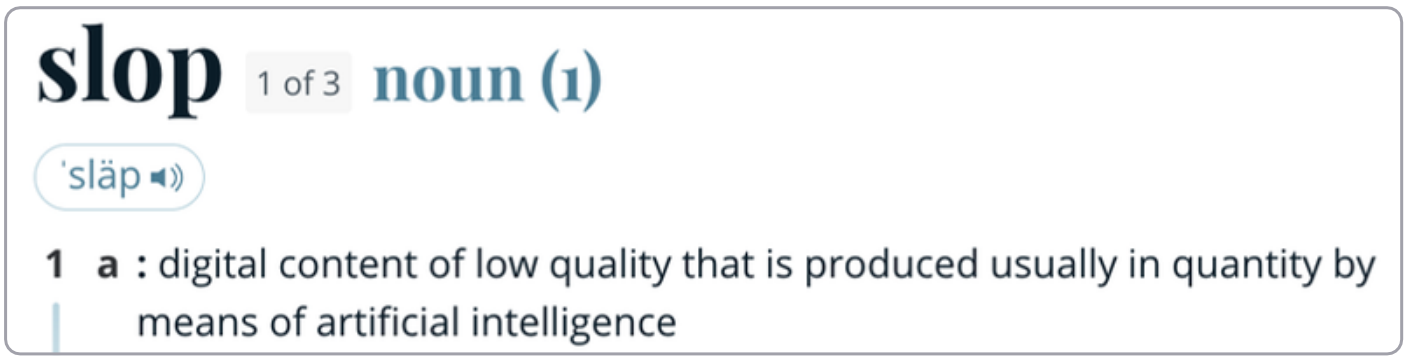
\includegraphics[width=.75\textwidth]{figs/slop.png}\\[6mm]
    {\fontfamily{ppl}\selectfont\color{muted}\LARGE Merriam-Webster\\
      \Large 2025 Word of the Year}
  \end{center}
  \vfill
\end{frame}

% ================================================================ 22. Doorstep
\begin{frame}
  \statement{I don't want to drop slop at your doorstep\\[8mm]
    I welcome guidance to make\\this a proper contribution}
\end{frame}

% ================================================================ 23. Evidence
\begin{frame}{Evidence}
  \statement{ACL2 books certify\\[2mm]
    SpecTest3 suite: 99.98\%\\[2mm]
    \muted{64,005 examples pass, 13 fail}}
\end{frame}

% ================================================================ 24-28. Demo
\begin{frame}
  \statement{\Huge Demo}
\end{frame}

\newcommand{\fullbleed}[1]{%
  \begin{frame}[plain]
    \begin{tikzpicture}[remember picture,overlay]
      \node[inner sep=0] at (current page.center)
        {\includegraphics[width=\paperwidth]{#1}};
    \end{tikzpicture}
  \end{frame}}
\fullbleed{figs/sem-demo1.png}
\fullbleed{figs/sem-demo2.png}
\fullbleed{figs/sem-demo3.png}
\fullbleed{figs/sem-demo4.png}

% ================================================================ 29. Thanks to
\begin{frame}{Acknowledgements}
  \statement{Jim White, testing and encouragement\\[4mm]
    OpenHands, my employer during phase 1}
\end{frame}

% ================================================================ 30. Thank you
{\setbeamertemplate{footline}{}
\begin{frame}
  \statement{{\Huge Thank you}\\[14mm]
    \link{github.com/raymyers/wasm-acl2}\\[2mm]
    \link{raymyers.org}}
\end{frame}}

\end{document}
